% this file should contain a summary of the propulsion system analysis tools and models including propeller, electric and cycle

% Summary paragraph
The propulsion systems under consideration for NASA's UAM concept vehicles cover a range of different system configurations from all-electric to turbo-electric architectures.
While the various concept vehicles consider different propulsion systems, the systems all contain similar elements leading to the developement of three supporting analysis tools and models.
These tools and models include those for the rotor or propeller, electrical system and gas turbine thermodynamic cycle, which are described in this section.  
For the tiltwing vehicle examined in this study, these three models were combined to form a propulsion system model as shown in Figure \ref{f:turboelectric}. 

\begin{figure}
\begin{center}
 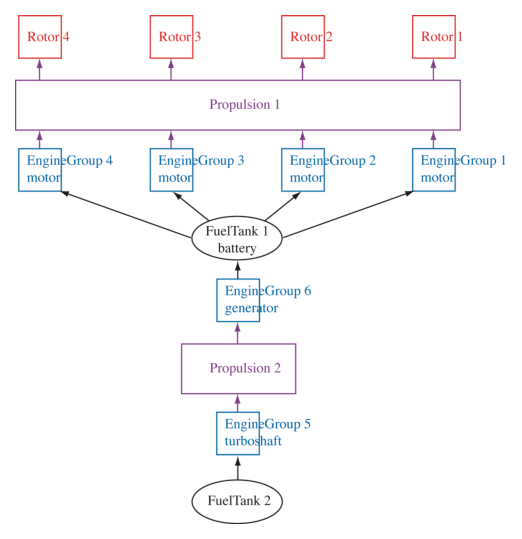
\includegraphics[width=0.6\textwidth]{../Images/Turboelectric.pdf}
 \caption{Tiltwing Aircraft Turboelectric Propulsion System.\cite{johnson2018concept}}
 \label{f:turboelectric}
\end{center}
\end{figure}

\subsubsection{Propeller Analysis} %Dan
This section needs a short summary of the propeller analysis in OpenBEMT
\begin{itemize}
    \item Describe the analysis tool and summarize the physics captured by the tool
    \item Describe the inputs and outputs of the code
    \item Make sure to include both design/static information as well as ODE information as appropriate
    \item Reference previous publications on the tool
    \item Describe the model created using the tool for the tiltwing UAM vehicle (include graphic as needed)
\end{itemize}

\subsubsection{Electrical System Analysis} %Eric



To model the electrical components of the propulsion system, a load flow analysis capability was developed on top of the OpenMDAO framework.
Load flow analysis is traditionally used by power engineers to model interconnected electrical systems such as the terrestrial AC power grid.  
However, it has also been extended to analyze DC and hybrid AC-DC systems\cite{ahmed2018generalized} as well as isolated micro-grids.
One of the benefits of the load flow method for EAP concepts is that it predicts voltages and currents throughout an electrical network given the states of distributed electric generators and loads.
This tool is actively in development and the resulting capability will be documented in a separate paper at this same conference.\cite{hendricks2019load}

\subsubsection{Thermodynamic Cycle Analysis} %Jeff, Eric
To model the gas turbine portions of the propulsion system, the recently developed thermodynamic cycle analysis tool pyCycle was selected.\cite{gray2017chemical,hearn2016optimization}
PyCycle is a new analysis tool being developed at NASA Glenn Research Center within the OpenMDAO framework.
While PyCycle is similar to other cycle analysis tools such as NPSS, its unique capability is that it provides analytic derivatives to better support gradient based solvers and optimizers.  
% This capability is enabled by developing the analysis tool within the OpenMDAO framework and taking advantage of the unified derivative methodology. 
pyCycle has been demonstrated in the context of a trajectory optimization in a previous research effort\cite{hendricks2017simultaneous} and the development of a turboshaft engine for the UAM turboelectric tiltwing aircraft will be published a this same conference.\cite{chapman2018multi}
The engine components comprising the turboshaft model for the tiltwing aircraft are shown in Figure \ref{f:turboshaft}.

\begin{figure}
\begin{center}
 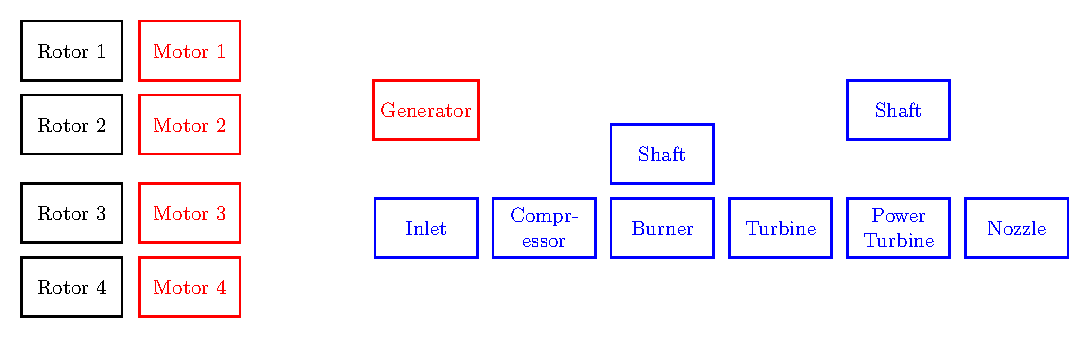
\includegraphics[scale=1.0]{../Images/Propulsion_system.pdf}
 \caption{Block Diagram of pyCycle Turboshaft Model.\cite{chapman2018multi}}
 \label{f:turboshaft}
\end{center}
\end{figure}

